%!TEX root = ../../main.tex

\subsection{Clustering Features}
\label{collection:clustering}

The content similarity between a target and candidate event is a potentially very useful feature for merging events that discuss the same real-world event.
Similarly to how many event detection approaches define tweet similarity, we define event content similarity as the cosine of the angle between the term frequency vectors for the target event and candidate event:
\begin{equation}
	S_t = cos(e_t, e'_t)
\end{equation}
where vectors $e_t$ and $e'_t$ contain counts for the top 10 most frequent terms (after stemming and stopword removal) for all tweets in the target and candidate events respectively.

We note that in certain cases, a target and candidate event may have very low content similarity despite discussing the same real-world event.
This is particularity common for events from the same detection approach, where the tweet text has already been used to perform clustering.
This can result in several clusters discussing the same real-world event, often with very dissimilar content, making it difficult to identify any relationship based on content alone.
For example, again using the presidential debate as an example, the quote ``Well, Governor, we also have fewer horses and bayonets, because the nature of our military's changed.'' was extremely popular and relevant to the debate itself, however, matching this back to the election is very difficult if the context is not known, and using only tweet content based features to match it to other clusters is very difficult.
This means that we cannot rely only on tweet content features when performing event clustering.

Fortunately, for both Event Detection and Wikipedia events, we also have the  descriptions given by annotators for each of the events.
Since the descriptions are often (but not always) higher level than the tweets, they are more likely to provide useful information for linking two events.
Thus, we define the description similarity, $S_d$, as the cosine of the angle between the term frequency vectors of the descriptions for the target and candidate events:
\begin{equation}
	S_d = cos(e_d, e'_d)
\end{equation}
where the vectors $e_d$ and $e'_d$ contain term counts (after stemming and stopword removal) for all descriptions given by annotators for the target and candidate events respectively.

Manual inspection of the descriptions shows that the vast majority contain at least one named entity (such as a person, location or organization), and many descriptions contain only a name entity with no other descriptive terms.
We also note that, in cases where the descriptions describe different aspects of the same real-world event, often the only constant is the mention of a named entity or named entities.
Of the 20 or so events that discuss Felix Baumgartner's record-breaking space jump, many of the descriptions  focus on particular moments before, during or after the jump. For example, one description given for tweets discussing his ascent reads: ``Felix Baumgartner is ready to jump from a height that no one has ever done'', while one given for tweets discussing his successful landing: ``felix baumgartner breaks world record free fall''.
Although both describe the same real-world event, they are different moments in time, and the descriptions given contain no overlapping terms other than the name of the person involved.
This is a common occurrence for events that were followed in real-time, particularity broadcast events watched by many users with many different subtopics.
This can make it difficult to use annotator descriptions to measure event similarity, as although they may describe the same real-world event, the descriptions can be quite dissimilar depending on the granularity of the events.
To solve this, rather than rely purely on description similarity, we also calculated the named entity similarity $S_n$, and take the maximum value for either $S_n$ or $S_d$ as the annotation similarity, $S_a$:
\begin{align*}
	S_n &= cos(e_n, e'_n) & S_a &= max(S_n, S_d) \numberthis
\end{align*}
where $e_n$ ad $e'_n$ are the entity frequency vectors containing counts for each named entity mentioned in the annotator descriptions (extracted using the NLTK 2.0.5 Python library with default English models) for target event $e$ and candidate event $e'$.
Taking the maximum similarity of the two allows us to optimize for the two cases: (i) when the descriptions describe an event at the same level of granularity (often the case for events from different sources) the full description can be used, however when events are described at different levels of granularity or at different moments in time, entity similarity can be used.

\subsubsection{Categories}
As described in section \ref{collection:sec:annotation}, for each event, we asked annotators to select the category that best fit the event from the 13 categories used by the TDT project.
Annotator agreement across categories was substantial (\(k = 0.76\)), however closer examination of the annotations raises a number of potential issues that could effect the usefulness of categories for clustering.
Using the third U.S. Presidential Debate as an example of a large event with many different subtopics, we note that the LSH approach produced over 40 clusters discussing various sub-events and topics within the debate.
Many of the subjects of the debate were related to economics, business and international relations.
This is an issue because annotators often categorized events using only the topic of discussion (e.g. New Laws, Political or Diplomatic Meetings), rather than the the specific real world event, in this case, the debate as part of the U.S Presidential Election (which would fall under the TDT category Elections).
Despite it being clear at a high level that the debate should be categorized as Election, it is not as clear when looking at the specific subtopics within the debate --- the categorization changes as the level of granularity is changed.
Similarly, the Wikipedia Current Events Portal assigns a category to each event, however these categories are often very low-level and specific, such as `History', `Literature', and `Spirituality'.

\begin{table}
	\centering
	\caption{Combined categories with their corresponding TDT and Wikipedia categories}
	\label{collection:table:catTable}

	\footnotesize
	\begin{tabulary}{\textwidth}{lLL}
	\toprule
	\textbf{Combined} & \textbf{TDT Categories} & \textbf{Wikipedia Categories}  \\
	\midrule
	Armed Conflicts and Attacks & Acts of Violence or War & Armed conflicts, Attacks \\
	\midrule
	Arts, Culture and Entertainment & Celebrity and Human Interest News & Arts, Culture, Literature, Religion, Spirituality \\
	\midrule
	Business and Economy & Financial News & Business, Economics \\
	\midrule
	Disasters and Accidents & Accidents, Natural Disaster & Accidents, Disasters \\
	\midrule
	Law, Politics and Scandals & Elections, Political and Diplomatic Meetings, Legal / Criminal Cases, New Laws, Scandals / Hearings & International relations, Human rights, Law, Crime, Politics, Elections \\
	\midrule
	Sports & Sports News & Sports \\
	\midrule
	Science and Technology & Science and Discovery News & Exploration, Innovation, Science, Technology \\
	\midrule
	Miscellaneous & Miscellaneous News & \emph{Anything not listed above. e.g. Heath, Transport}  \\
	\bottomrule
	\end{tabulary}

\end{table}

Before we can use the TDT and Wikipedia categories as a feature for clustering, we must create a mapping between them.
Simply creating a direct mapping between TDT categories and Wikipedia categories would solve the mapping problem but not increase agreement between the annotations from the event detection approaches.
Thus, we created a new set of categories, each of which covers a much broader range than either the TDT or Wikipedia categories.
Table~\ref{collection:table:catTable} shows the new categories and the corresponding categories from the TDT project and Wikipedia.
Re-computing annotator agreement for the event detection event annotation after mapping the TDT categories to the combined categories shows an improvement from  $k = 0.76$ to $k = 0.81$.
This is a good indication that our combined categories improve categorization and should help to make categories a more effective feature for clustering.

We compute the category similarity $S_c$ between events $e$ and $e'$ as as the cosine of the angle in vector space between their category frequency vectors ($e_c$ and $e'_c$ respectively):
\begin{equation}
	S_c = cos(e_c, e'_c)
\end{equation}
Category frequency vectors $e_c$ and $e'_c$ are counts of how frequently a category was selected by annotators for a given event (after mapping to combined categories). For events from Wikipedia, the vector simply contained a 1 for the category given by Wikipedia (after mapping to the combined categories).
Since cosine is already length normalized, it is not necessary to perform any sort of length or weight adjustments to the vectors.

\subsubsection{Temporal Proximity}
Temporal proximity is extremely important in the clustering of events -- events which have a significant period of time between them are unlikely to be related to the same real-world event.
For example, the three U.S. Presidential Debates are all likely to be very similar in terms of category features content-based features.
The largest differentiating factor is the specific time when the events took place.

On the other hand, events which share similar characteristics in terms of both category and content-based features are still relatively common in the same temporal region.
Sports events are an example of this type of event --- it is not uncommon for two football matches to occur simultaneously, such as World Cup qualifying matches.
These share the same category, will have similar content, and overlap in time, making them particular difficult to distinguish.

Taking this into consideration, we chose not to use temporal proximity as a measure of similarity.
Rather, we use it as a filter, and say that events which are more than $T$ hours apart cannot be merged.

\subsection{Clustering Algorithm}
\label{sec:clusteringalg}
For each event \(e\), our algorithm calculates its similarity $S_f$ against every candidate event \(e'\) within a time window of 6 hours.
The similarity is calculated as so:
\begin{equation} \label{eq:simcluster}
S_{f} = (0.3 * S_{t}) + (0.3 * S_{c}) + (0.4 * S_{a})
\end{equation}
If two events are found to have an \(S_{f}\) value above 0.5 then they are clustered together (merged).
If both \(e\) and \(e'\) already have clusters then the two clusters are merged.
The pseudo-code for our clustering approach is shown in Algorithm~\ref{alg:clustering}.

\begin{algorithm}[t!]
$clustered$ = $\emptyset$\;
\ForEach{event e in targets} {
	add $e$ to $clustered$\;
	\ForEach{event e' in candidates} {

		$S_{a}$ = $max\{cos(e_d, e'_d), cos(e_n, e'_n)\}$\;
		$S_{c}$ = $cos(e_c, e'_c)$\;
		$S_{t}$ = $cos(e_t, e'_t)$\;
		$S_{f}$ = $(0.3 * S_{t}) + (0.c * S_{c}) + (0.4 * S_{a})$\;
		\If{$S_{f}$ \(\ge\) 0.5 and $time\_diff(e, e')$ \(\le\) $T$} {
			\uIf{neither e nor e' have clusters}{
				create new cluster containing e and e'\;
			} \eIf{both e and e' have clusters}{
				merge cluster(e) and cluster(e')\;
			}{
				add e or e' to existing cluster\;
			}
		}
	}
}
\caption{Pseudocode for our event clustering approach}
\label{alg:clustering}
\end{algorithm}

Parameter weights were optimized by varying between 0.0 and 1.0 in steps of 0.1, such that the sum of all weights was 1.0.
The weights given in equation \ref{eq:simcluster} gave the highest B-Cubed precision (0.92) and recall (0.86) values (F1 = 0.86).
The maximum time difference, $T$, was set to 6 hours  as only a 3.4\% of events were matched outside of a 6 hour window, as show in Figure~\ref{fig:dif_diff}.
This allows for lag between events, whilst still giving a reasonable guarantee that the events generated will fit our definition of event.

\begin{figure}
	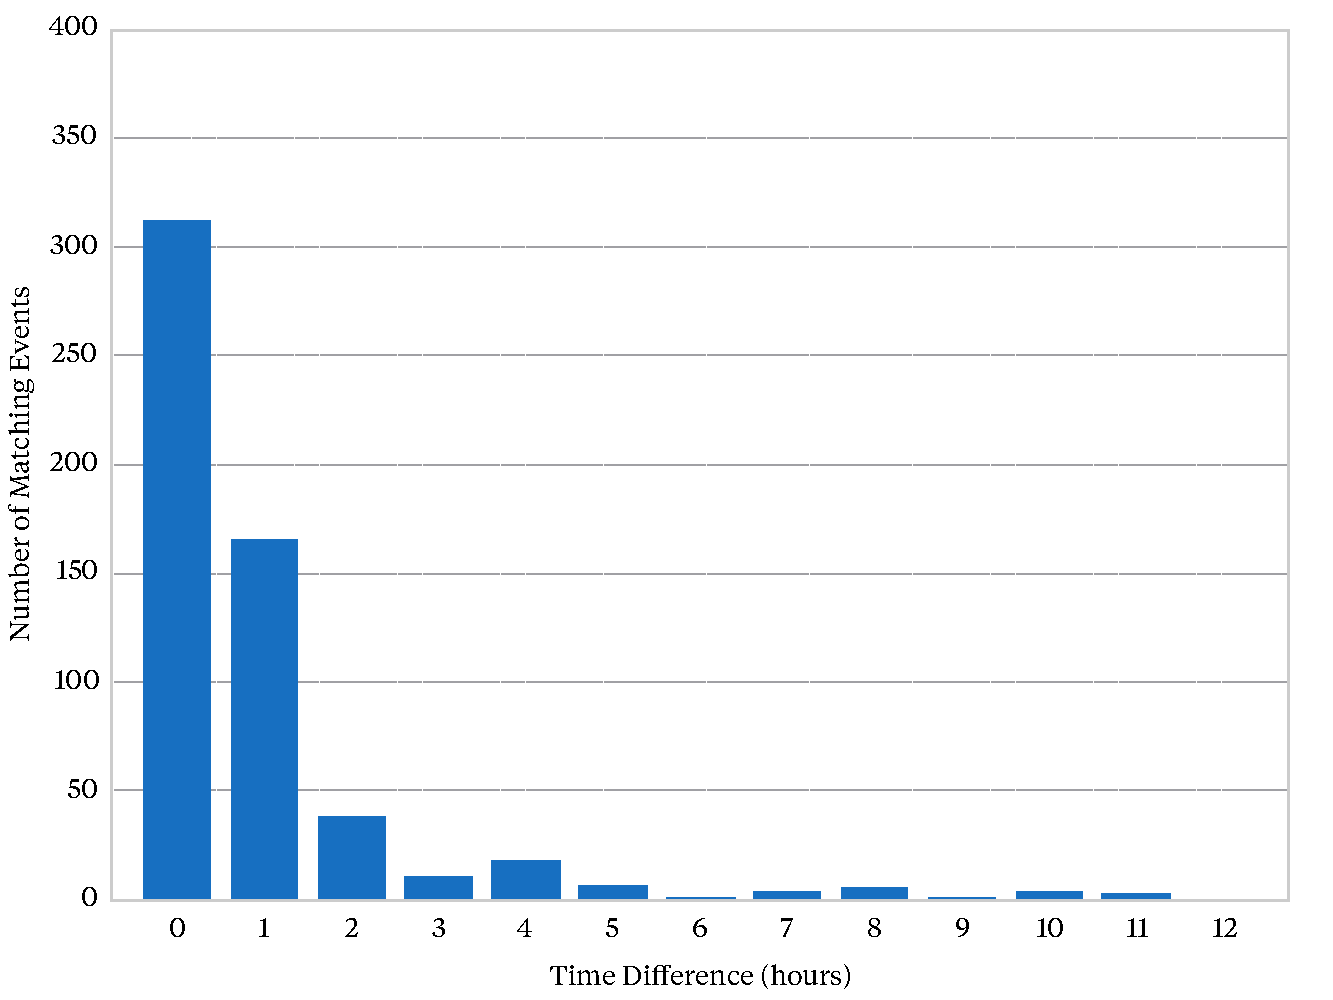
\includegraphics[width=\textwidth]{./Chapters/Collection/images/times}
	\caption{The distribution of times between matched events, based upon the number of hours between the centroid times of the events}
	\label{fig:dif_diff}
\end{figure}
